\documentclass[border=0mm,tikz]{standalone}


\usepackage{cmap}
% \usepackage[defaultsans]{droidsans}
% \renewcommand*\familydefault{\sfdefault} %% Only if the base font of the document is to be typewriter style
\usepackage[T2A]{fontenc}
\usepackage[utf8x]{inputenc}
\usepackage{amsmath,amssymb}
\usepackage{esdiff,esint}


\usepackage{pgfplots}
\usetikzlibrary{shapes, arrows}
\pgfplotsset{compat=1.10}
\usepgfplotslibrary{fillbetween}
\usetikzlibrary{patterns}
\usepackage[outline]{contour}

\def\centerarc[#1](#2)(#3:#4:#5);%
%Syntax: [draw options] (center) (initial angle:final angle:radius)
    {
    %\draw[#1] ($(#2)+({#5*cos(#3)},{#5*sin(#3)})$) arc (#3:#4:#5);
    \draw[#1]([shift=(#3:#5)]#2) arc (#3:#4:#5);
    }
\usetikzlibrary{quotes,angles}
\begin{document}

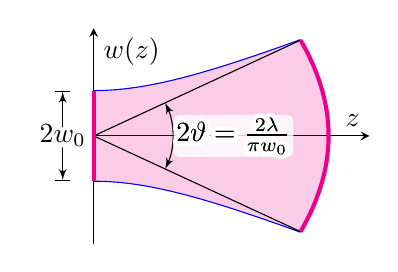
\begin{tikzpicture}%width=12cm,height=8cm]
\begin{axis}[axis lines=middle,
            xlabel={$z$},
            ylabel={$w(z)$},
            scale=0.8,
            width=7cm,
            height=5cm,
            % enlargelimits,
            % unit vector ratio*=0.42 1.5 1,
            ytick=\empty,
            xtick=\empty,
            ymin=-0.95,
            ymax=0.95,
            xmin=-1.9,
            xmax=8,
            % disabledatascaling,
            % domain=-2:2, 
            % restrict y to domain=-2:2,
            % xtick={1,4},
            % xticklabels={a,b}
            ]


% \xdef\From{0.5}
% \xdef\To{3}

% \path[name path=axisy] (axis cs:0,-2) -- (axis cs:0,2);
% \path[name path=axisx] (axis cs:-\To,0) -- (axis cs:\To,0);
% \path[name path=xmin] (axis cs:-\To,-2) -- (axis cs:\To,-2); 
% \path[name path=xmax] (axis cs:-\To,2) -- (axis cs:\To,2);

\xdef\wo{0.4}
\xdef\coeff{0.05}

\contourlength{0.6mm};
\addplot[name path=A,blue,domain={0:6},samples=100] {\wo*sqrt(1+(\coeff*x/\wo^2)^2)} node[pos=.8, above]{};

\addplot[name path=B,blue,domain={0:6},samples=100] {-\wo*sqrt(1+(\coeff*x/\wo^2)^2)} node[pos=.8, above]{};

\addplot[fill=magenta, opacity=0.2]fill between[of=A and B, soft clip={domain=0:6}];

\xdef\Z{6}
\pgfmathparse{tan(180/3.14*\coeff/\wo)*\Z*1.12}\let\H\pgfmathresult
\draw (axis cs:0,0) coordinate (0) -- (axis cs:\Z,\H) coordinate (A);
\draw (axis cs:0,0) -- (axis cs:\Z,-\H) coordinate (B);

\draw[white, very thick] (axis cs:-2,0) -- (axis cs:0,0); 
\draw [thick, magenta, line width=1.5pt,name path=C] (A) to [out=-60, in=60] (B);
\draw [thick, magenta, line width=1.5pt] (axis cs:0,-\wo) -- (axis cs:0,\wo);

\path[name path=D] (A) -- (B);

\addplot[fill=magenta, opacity=0.2]fill between[of=C and D];

\draw (axis cs:0,0) pic[draw=black, <->,>=latex', angle eccentricity=1.2, angle radius=1cm]
    {angle=B--0--A};

\draw (axis cs:2.3,0) node[right,fill=white,rounded corners=2pt,inner sep=1pt,fill opacity=0.8] {\contour{white}{$2\vartheta=\frac{2\lambda}{\pi w_0}$}};

\draw (axis cs:2.3,0) node[right,rounded corners=2pt,inner sep=1pt,] {{$2\vartheta=\frac{2\lambda}{\pi w_0}$}};
% \pgfmathparse{1*(\Z*(1+(\wo^2/(\coeff*\Z))^2))}\let\Radius\pgfmathresult
% \pgfmathparse{atan(\H)}\let\angle\pgfmathresult
\xdef\Radius{1}
\xdef\angle{70}
\pgfmathparse{6-\Radius}\let\coo\pgfmathresult
\centerarc[](5.5,0)(-\angle:\angle:\Radius);
% \draw[dashed] (axis cs:{-1},{exp(-1)}) -- (axis cs:{-2.5},{exp(-1)});



\draw[|<->|,>=latex'] (axis cs:-0.9,-\wo) -- node[pos=0.5] {\contour{white}{$2w_0$}} (axis cs:-0.9,\wo);


% \draw[|<->|,>=latex'] (axis cs:{-2.4},{0}) -- node[pos=0.55] {\contour{white}{$E_0/e$}} (axis cs:{-2.4},{exp(-1)});

% \draw[|<->|,>=latex'] (axis cs:{2.4},{0}) -- node[pos=0.5] {\contour{white}{$E_0$}} (axis cs:{2.4},{1});

% \draw[dashed] (axis cs:{2.5},{1}) -- (axis cs:{0},{1});
% \addplot[name path=B,blue,domain={-\To:-\From},samples=100] {1/x} node[pos=.8, above]{};

% \addplot[pattern=north east lines, pattern color=black!50]fill between[of=B and xmin, soft clip={domain=-\To:-\From}];

% \addplot[pattern=north east lines, pattern color=black!50]fill between[of=A and xmax, soft clip={domain=\From:\To}];

% \addplot[pattern=north east lines, pattern color=black!50]fill between[of=axisx and xmin, soft clip={domain=0:\To}];

% \addplot[pattern=north east lines, pattern color=black!50]fill between[of=axisx and xmax, soft clip={domain=-\To:0}];

% \draw [densely dashed, opacity=0.3] (axis cs:-2,-2) -- (axis cs:2,2);

% \draw[dashed] (axis cs:-1,0) 
%       -- (axis cs:-1,-1)
%       -- (axis cs:0,-1);

% \draw[dashed] (axis cs:1,0) 
%       -- (axis cs:1,1)
%       -- (axis cs:0,1);


% % \contourlength{1cm}; 


% \coordinate (parallel)  at (axis cs:2,1.5);
% \coordinate (ust)  at (axis cs:-1.5,1);
% \coordinate (conc)  at (axis cs:-2.1,-1.5);
% \coordinate (conf)  at (axis cs:1.5,-1);

% \xdef\Scale{1}
% % \contour{white}{}
% \node[scale=1.1,align=center] at (ust)  {\contour{white}{Условие устойчивости:}\\\contour{white}{$0<g_1g_2<1$}\\\\\contour{white}{где}\\\\\contour{white}{$g_1=1-\frac{d}{R_1},\quad g_2=1-\frac{d}{R_2}$}};


% \draw (parallel) node[scale=\Scale,align=center]  {\contour{white}{Плоские зеркала}\\\contour{white}{($R_1=R_2=\infty$)}}
% node[inner sep=0pt, yshift=-1.5em, below] at (parallel)
%     {\includegraphics[width=7em]{parallel}};


% \draw (conc) node[scale=\Scale,align=center]  {\contour{white}{Концентрические}\\\contour{white}{зеркала}\\\contour{white}{($R_1=R_2=d/2$)}} node[above,inner sep=0pt,yshift=1.7em] 
%     {\includegraphics[width=7em]{conc}};



% \draw (conf) node[inner sep=0pt,above]
%     {\includegraphics[width=7em]{conf}} node [below, align=center,scale=\Scale] {\contour{white}{Конфокальные}\\\contour{white}{зеркала}\\\contour{white}{($R_1=R_2=d$)}};
% % \node[coordinate,pin=30:{$A$}] at (axis cs:3.8,3){};

% \coordinate (A) at (axis cs:0.7,-0.75);
% \coordinate (0) at (axis cs:0,0);
% % \draw (A) -- (0);
% \path[draw] (A) edge [out=180, in=-80,->, thick, >=latex] (0);

% \draw[fill=magenta] (axis cs:0,0) circle (2pt);

% \draw[fill=magenta] (axis cs:1,1) circle (2pt) node[left, yshift=-1em, scale=0.8]{\contour{white}{$(1,1)$}};

% \draw[fill=magenta] (axis cs:-1,-1) circle (2pt) node[right, yshift=1em, scale=0.8]{\contour{white}{$(-1,-1)$}};

\end{axis}
\end{tikzpicture}

% \begin{tikzpicture}
% \begin{axis}[axis lines=middle,
%             xlabel=$x$,
%             ylabel=$y$,
%             enlargelimits,
%             ytick=\empty,
%             xtick={-2.19,2.19},
%             xticklabels={$x_1$,$x_2$}]
% \addplot[name path=F,blue,domain={-4:4}] {-(1/6)*x^2+2} node[pos=1, below]{$f$};

% \addplot[name path=G,green,domain={-4:4}] {0.25*x^2}node[pos=1, above]{$g$};

% \addplot[pattern=north west lines, pattern color=brown!50]fill between[of=F and G, soft clip={domain=-2.19:2.19}]
% ;
% \node[coordinate,pin=60:{$A$}] at (axis cs:1.1,1.6){};

% \end{axis}
% \end{tikzpicture}
\end{document}